\PassOptionsToPackage{unicode=true}{hyperref} % options for packages loaded elsewhere
\PassOptionsToPackage{hyphens}{url}
%
\documentclass[]{article}
\usepackage{lmodern}
\usepackage{amssymb,amsmath}
\usepackage{ifxetex,ifluatex}
\usepackage{fixltx2e} % provides \textsubscript
\ifnum 0\ifxetex 1\fi\ifluatex 1\fi=0 % if pdftex
  \usepackage[T1]{fontenc}
  \usepackage[utf8]{inputenc}
  \usepackage{textcomp} % provides euro and other symbols
\else % if luatex or xelatex
  \usepackage{unicode-math}
  \defaultfontfeatures{Ligatures=TeX,Scale=MatchLowercase}
\fi
% use upquote if available, for straight quotes in verbatim environments
\IfFileExists{upquote.sty}{\usepackage{upquote}}{}
% use microtype if available
\IfFileExists{microtype.sty}{%
\usepackage[]{microtype}
\UseMicrotypeSet[protrusion]{basicmath} % disable protrusion for tt fonts
}{}
\IfFileExists{parskip.sty}{%
\usepackage{parskip}
}{% else
\setlength{\parindent}{0pt}
\setlength{\parskip}{6pt plus 2pt minus 1pt}
}
\usepackage{hyperref}
\hypersetup{
            pdftitle={Lecture 2 in class},
            pdfauthor={Jung-Jin Lee},
            pdfborder={0 0 0},
            breaklinks=true}
\urlstyle{same}  % don't use monospace font for urls
\usepackage[margin=1in]{geometry}
\usepackage{color}
\usepackage{fancyvrb}
\newcommand{\VerbBar}{|}
\newcommand{\VERB}{\Verb[commandchars=\\\{\}]}
\DefineVerbatimEnvironment{Highlighting}{Verbatim}{commandchars=\\\{\}}
% Add ',fontsize=\small' for more characters per line
\usepackage{framed}
\definecolor{shadecolor}{RGB}{248,248,248}
\newenvironment{Shaded}{\begin{snugshade}}{\end{snugshade}}
\newcommand{\AlertTok}[1]{\textcolor[rgb]{0.94,0.16,0.16}{#1}}
\newcommand{\AnnotationTok}[1]{\textcolor[rgb]{0.56,0.35,0.01}{\textbf{\textit{#1}}}}
\newcommand{\AttributeTok}[1]{\textcolor[rgb]{0.77,0.63,0.00}{#1}}
\newcommand{\BaseNTok}[1]{\textcolor[rgb]{0.00,0.00,0.81}{#1}}
\newcommand{\BuiltInTok}[1]{#1}
\newcommand{\CharTok}[1]{\textcolor[rgb]{0.31,0.60,0.02}{#1}}
\newcommand{\CommentTok}[1]{\textcolor[rgb]{0.56,0.35,0.01}{\textit{#1}}}
\newcommand{\CommentVarTok}[1]{\textcolor[rgb]{0.56,0.35,0.01}{\textbf{\textit{#1}}}}
\newcommand{\ConstantTok}[1]{\textcolor[rgb]{0.00,0.00,0.00}{#1}}
\newcommand{\ControlFlowTok}[1]{\textcolor[rgb]{0.13,0.29,0.53}{\textbf{#1}}}
\newcommand{\DataTypeTok}[1]{\textcolor[rgb]{0.13,0.29,0.53}{#1}}
\newcommand{\DecValTok}[1]{\textcolor[rgb]{0.00,0.00,0.81}{#1}}
\newcommand{\DocumentationTok}[1]{\textcolor[rgb]{0.56,0.35,0.01}{\textbf{\textit{#1}}}}
\newcommand{\ErrorTok}[1]{\textcolor[rgb]{0.64,0.00,0.00}{\textbf{#1}}}
\newcommand{\ExtensionTok}[1]{#1}
\newcommand{\FloatTok}[1]{\textcolor[rgb]{0.00,0.00,0.81}{#1}}
\newcommand{\FunctionTok}[1]{\textcolor[rgb]{0.00,0.00,0.00}{#1}}
\newcommand{\ImportTok}[1]{#1}
\newcommand{\InformationTok}[1]{\textcolor[rgb]{0.56,0.35,0.01}{\textbf{\textit{#1}}}}
\newcommand{\KeywordTok}[1]{\textcolor[rgb]{0.13,0.29,0.53}{\textbf{#1}}}
\newcommand{\NormalTok}[1]{#1}
\newcommand{\OperatorTok}[1]{\textcolor[rgb]{0.81,0.36,0.00}{\textbf{#1}}}
\newcommand{\OtherTok}[1]{\textcolor[rgb]{0.56,0.35,0.01}{#1}}
\newcommand{\PreprocessorTok}[1]{\textcolor[rgb]{0.56,0.35,0.01}{\textit{#1}}}
\newcommand{\RegionMarkerTok}[1]{#1}
\newcommand{\SpecialCharTok}[1]{\textcolor[rgb]{0.00,0.00,0.00}{#1}}
\newcommand{\SpecialStringTok}[1]{\textcolor[rgb]{0.31,0.60,0.02}{#1}}
\newcommand{\StringTok}[1]{\textcolor[rgb]{0.31,0.60,0.02}{#1}}
\newcommand{\VariableTok}[1]{\textcolor[rgb]{0.00,0.00,0.00}{#1}}
\newcommand{\VerbatimStringTok}[1]{\textcolor[rgb]{0.31,0.60,0.02}{#1}}
\newcommand{\WarningTok}[1]{\textcolor[rgb]{0.56,0.35,0.01}{\textbf{\textit{#1}}}}
\usepackage{graphicx,grffile}
\makeatletter
\def\maxwidth{\ifdim\Gin@nat@width>\linewidth\linewidth\else\Gin@nat@width\fi}
\def\maxheight{\ifdim\Gin@nat@height>\textheight\textheight\else\Gin@nat@height\fi}
\makeatother
% Scale images if necessary, so that they will not overflow the page
% margins by default, and it is still possible to overwrite the defaults
% using explicit options in \includegraphics[width, height, ...]{}
\setkeys{Gin}{width=\maxwidth,height=\maxheight,keepaspectratio}
\setlength{\emergencystretch}{3em}  % prevent overfull lines
\providecommand{\tightlist}{%
  \setlength{\itemsep}{0pt}\setlength{\parskip}{0pt}}
\setcounter{secnumdepth}{0}
% Redefines (sub)paragraphs to behave more like sections
\ifx\paragraph\undefined\else
\let\oldparagraph\paragraph
\renewcommand{\paragraph}[1]{\oldparagraph{#1}\mbox{}}
\fi
\ifx\subparagraph\undefined\else
\let\oldsubparagraph\subparagraph
\renewcommand{\subparagraph}[1]{\oldsubparagraph{#1}\mbox{}}
\fi

% set default figure placement to htbp
\makeatletter
\def\fps@figure{htbp}
\makeatother


\title{Lecture 2 in class}
\author{Jung-Jin Lee}
\date{1/14/2020}

\begin{document}
\maketitle

\begin{Shaded}
\begin{Highlighting}[]
\NormalTok{first_name <-}\StringTok{ }\KeywordTok{c}\NormalTok{(}\StringTok{"Lisa"}\NormalTok{, }\StringTok{"John"}\NormalTok{, }\StringTok{"Chuck"}\NormalTok{, }\StringTok{"Matt"}\NormalTok{)}
\NormalTok{last_name <-}\StringTok{ }\KeywordTok{c}\NormalTok{(}\StringTok{"Simpson"}\NormalTok{, }\StringTok{"Smith"}\NormalTok{, }\StringTok{"Williams"}\NormalTok{, }\StringTok{"June"}\NormalTok{)}
\NormalTok{age_yrs <-}\StringTok{ }\KeywordTok{c}\NormalTok{(}\DecValTok{8}\NormalTok{, }\DecValTok{42}\NormalTok{, }\DecValTok{81}\NormalTok{, }\DecValTok{23}\NormalTok{)}

\KeywordTok{length}\NormalTok{(first_name)}
\end{Highlighting}
\end{Shaded}

\begin{verbatim}
## [1] 4
\end{verbatim}

\begin{Shaded}
\begin{Highlighting}[]
\NormalTok{last_name[}\DecValTok{3}\NormalTok{]}
\end{Highlighting}
\end{Shaded}

\begin{verbatim}
## [1] "Williams"
\end{verbatim}

\begin{Shaded}
\begin{Highlighting}[]
\NormalTok{last_name[}\KeywordTok{c}\NormalTok{(}\DecValTok{3}\NormalTok{, }\DecValTok{4}\NormalTok{)]}
\end{Highlighting}
\end{Shaded}

\begin{verbatim}
## [1] "Williams" "June"
\end{verbatim}

\begin{Shaded}
\begin{Highlighting}[]
\NormalTok{book <-}\StringTok{ }\KeywordTok{data.frame}\NormalTok{(}\DataTypeTok{first =}\NormalTok{ first_name, }
                   \DataTypeTok{last =}\NormalTok{ last_name,}
                   \DataTypeTok{age =}\NormalTok{ age_yrs)}

\KeywordTok{dim}\NormalTok{(book)}
\end{Highlighting}
\end{Shaded}

\begin{verbatim}
## [1] 4 3
\end{verbatim}

\begin{Shaded}
\begin{Highlighting}[]
\KeywordTok{nrow}\NormalTok{(book)}
\end{Highlighting}
\end{Shaded}

\begin{verbatim}
## [1] 4
\end{verbatim}

\begin{Shaded}
\begin{Highlighting}[]
\KeywordTok{ncol}\NormalTok{(book)}
\end{Highlighting}
\end{Shaded}

\begin{verbatim}
## [1] 3
\end{verbatim}

\begin{Shaded}
\begin{Highlighting}[]
\KeywordTok{dim}\NormalTok{(book)}
\end{Highlighting}
\end{Shaded}

\begin{verbatim}
## [1] 4 3
\end{verbatim}

\begin{Shaded}
\begin{Highlighting}[]
\NormalTok{book[}\DecValTok{2}\NormalTok{, }\DecValTok{2}\NormalTok{]}
\end{Highlighting}
\end{Shaded}

\begin{verbatim}
## [1] Smith
## Levels: June Simpson Smith Williams
\end{verbatim}

\begin{Shaded}
\begin{Highlighting}[]
\NormalTok{book}\OperatorTok{$}\NormalTok{age}
\end{Highlighting}
\end{Shaded}

\begin{verbatim}
## [1]  8 42 81 23
\end{verbatim}

\begin{Shaded}
\begin{Highlighting}[]
\NormalTok{book[, }\DecValTok{3}\NormalTok{]}
\end{Highlighting}
\end{Shaded}

\begin{verbatim}
## [1]  8 42 81 23
\end{verbatim}

\begin{Shaded}
\begin{Highlighting}[]
\NormalTok{book[}\DecValTok{1}\OperatorTok{:}\DecValTok{3}\NormalTok{, }\DecValTok{2}\OperatorTok{:}\DecValTok{3}\NormalTok{]}
\end{Highlighting}
\end{Shaded}

\begin{verbatim}
##       last age
## 1  Simpson   8
## 2    Smith  42
## 3 Williams  81
\end{verbatim}

\begin{Shaded}
\begin{Highlighting}[]
\NormalTok{gender <-}\StringTok{ }\KeywordTok{c}\NormalTok{(}\StringTok{"Female"}\NormalTok{, }\StringTok{"Male"}\NormalTok{, }\StringTok{"Male"}\NormalTok{, }\StringTok{"Unknown"}\NormalTok{)}
\NormalTok{book}\OperatorTok{$}\NormalTok{sex <-}\StringTok{ }\NormalTok{gender}

\NormalTok{book}\OperatorTok{$}\NormalTok{remark <-}\StringTok{ "friend"}

\NormalTok{book}\OperatorTok{$}\NormalTok{extra <-}\StringTok{ }\KeywordTok{c}\NormalTok{(}\StringTok{"A"}\NormalTok{, }\StringTok{"B"}\NormalTok{)}

\NormalTok{df <-}\StringTok{ }\KeywordTok{data.frame}\NormalTok{(}\DataTypeTok{a =} \DecValTok{1}\OperatorTok{:}\DecValTok{6}\NormalTok{, }\DataTypeTok{b =} \StringTok{"some random"}\NormalTok{)}

\NormalTok{df}\OperatorTok{$}\NormalTok{third <-}\StringTok{ }\KeywordTok{c}\NormalTok{(}\StringTok{"aa"}\NormalTok{, }\StringTok{"bb"}\NormalTok{, }\StringTok{"cc"}\NormalTok{)}

\NormalTok{df}\OperatorTok{$}\NormalTok{fourth <-}\StringTok{ }\KeywordTok{c}\NormalTok{(}\StringTok{"xxx"}\NormalTok{, }\StringTok{"zzz"}\NormalTok{)}
\end{Highlighting}
\end{Shaded}

\begin{Shaded}
\begin{Highlighting}[]
\NormalTok{d <-}\StringTok{ }\KeywordTok{read.table}\NormalTok{(}\DataTypeTok{file =} \StringTok{"heights.txt"}\NormalTok{, }\DataTypeTok{header =} \OtherTok{TRUE}\NormalTok{, }\DataTypeTok{sep =} \StringTok{" "}\NormalTok{)}
\end{Highlighting}
\end{Shaded}

\begin{Shaded}
\begin{Highlighting}[]
\KeywordTok{dim}\NormalTok{(d)}
\end{Highlighting}
\end{Shaded}

\begin{verbatim}
## [1] 1375    2
\end{verbatim}

\begin{Shaded}
\begin{Highlighting}[]
\KeywordTok{names}\NormalTok{(d)}
\end{Highlighting}
\end{Shaded}

\begin{verbatim}
## [1] "Mheight" "Dheight"
\end{verbatim}

\begin{Shaded}
\begin{Highlighting}[]
\KeywordTok{head}\NormalTok{(d)}
\end{Highlighting}
\end{Shaded}

\begin{verbatim}
##   Mheight Dheight
## 1    59.7    55.1
## 2    58.2    56.5
## 3    60.6    56.0
## 4    60.7    56.8
## 5    61.8    56.0
## 6    55.5    57.9
\end{verbatim}

\begin{Shaded}
\begin{Highlighting}[]
\KeywordTok{tail}\NormalTok{(d)}
\end{Highlighting}
\end{Shaded}

\begin{verbatim}
##      Mheight Dheight
## 1370    69.5    70.4
## 1371    69.1    70.1
## 1372    65.0    71.6
## 1373    66.3    71.4
## 1374    70.8    71.0
## 1375    63.0    73.1
\end{verbatim}

\begin{Shaded}
\begin{Highlighting}[]
\NormalTok{vec <-}\StringTok{ }\DecValTok{1}\OperatorTok{:}\DecValTok{100}
\KeywordTok{head}\NormalTok{(vec)}
\end{Highlighting}
\end{Shaded}

\begin{verbatim}
## [1] 1 2 3 4 5 6
\end{verbatim}

\begin{Shaded}
\begin{Highlighting}[]
\KeywordTok{tail}\NormalTok{(vec)}
\end{Highlighting}
\end{Shaded}

\begin{verbatim}
## [1]  95  96  97  98  99 100
\end{verbatim}

\newpage

\hypertarget{some-sentence}{%
\subsection{Some sentence}\label{some-sentence}}

\hypertarget{another-sentence}{%
\subsubsection{Another sentence}\label{another-sentence}}

\begin{Shaded}
\begin{Highlighting}[]
\KeywordTok{library}\NormalTok{(tidyverse)}

\NormalTok{g1 <-}\StringTok{ }\KeywordTok{ggplot}\NormalTok{(d, }\KeywordTok{aes}\NormalTok{(}\DataTypeTok{x =}\NormalTok{ Mheight)) }\OperatorTok{+}\StringTok{ }
\StringTok{  }\KeywordTok{geom_histogram}\NormalTok{() }\OperatorTok{+}
\StringTok{  }\KeywordTok{theme_classic}\NormalTok{() }\OperatorTok{+}
\StringTok{  }\KeywordTok{ggtitle}\NormalTok{(}\StringTok{"Some fancy title"}\NormalTok{) }\OperatorTok{+}
\StringTok{  }\KeywordTok{xlab}\NormalTok{(}\StringTok{"some x axis name"}\NormalTok{) }\OperatorTok{+}
\StringTok{  }\KeywordTok{ylab}\NormalTok{(}\StringTok{"my first y axis name"}\NormalTok{)}

\KeywordTok{print}\NormalTok{(g1)}
\end{Highlighting}
\end{Shaded}

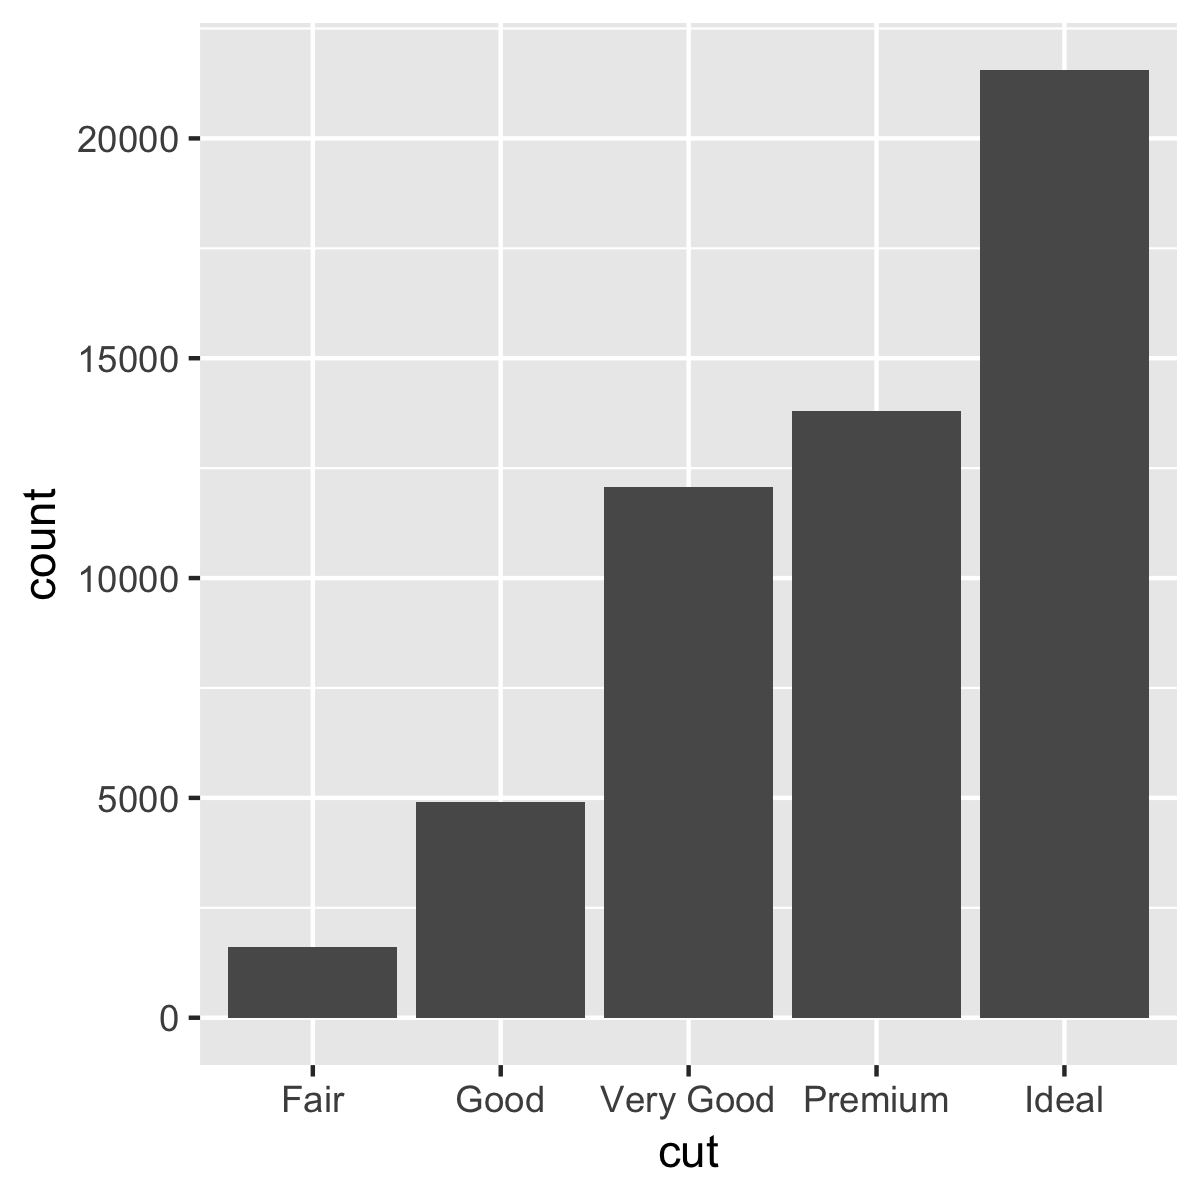
\includegraphics{lecture2_in_class_files/figure-latex/unnamed-chunk-5-1.pdf}

\begin{Shaded}
\begin{Highlighting}[]
\KeywordTok{library}\NormalTok{(tidyverse)}

\NormalTok{df <-}\StringTok{ }\NormalTok{diamonds }\CommentTok{## diamonds comes with ggplot2}
\KeywordTok{dim}\NormalTok{(df)}
\end{Highlighting}
\end{Shaded}

\begin{verbatim}
## [1] 53940    10
\end{verbatim}

\begin{Shaded}
\begin{Highlighting}[]
\NormalTok{g <-}\StringTok{ }\KeywordTok{ggplot}\NormalTok{(}\DataTypeTok{data =}\NormalTok{ df, }\KeywordTok{aes}\NormalTok{(}\DataTypeTok{x =}\NormalTok{ cut)) }\OperatorTok{+}\StringTok{ }
\StringTok{  }\KeywordTok{geom_bar}\NormalTok{() }\OperatorTok{+}\StringTok{ }
\StringTok{  }\KeywordTok{ggtitle}\NormalTok{(}\StringTok{"Whatever you like as a title"}\NormalTok{) }\OperatorTok{+}
\StringTok{  }\KeywordTok{xlab}\NormalTok{(}\StringTok{"Diamond cuts"}\NormalTok{) }\OperatorTok{+}
\StringTok{  }\KeywordTok{ylab}\NormalTok{(}\StringTok{"Number (Frequency)"}\NormalTok{) }

\KeywordTok{print}\NormalTok{(g)}
\end{Highlighting}
\end{Shaded}

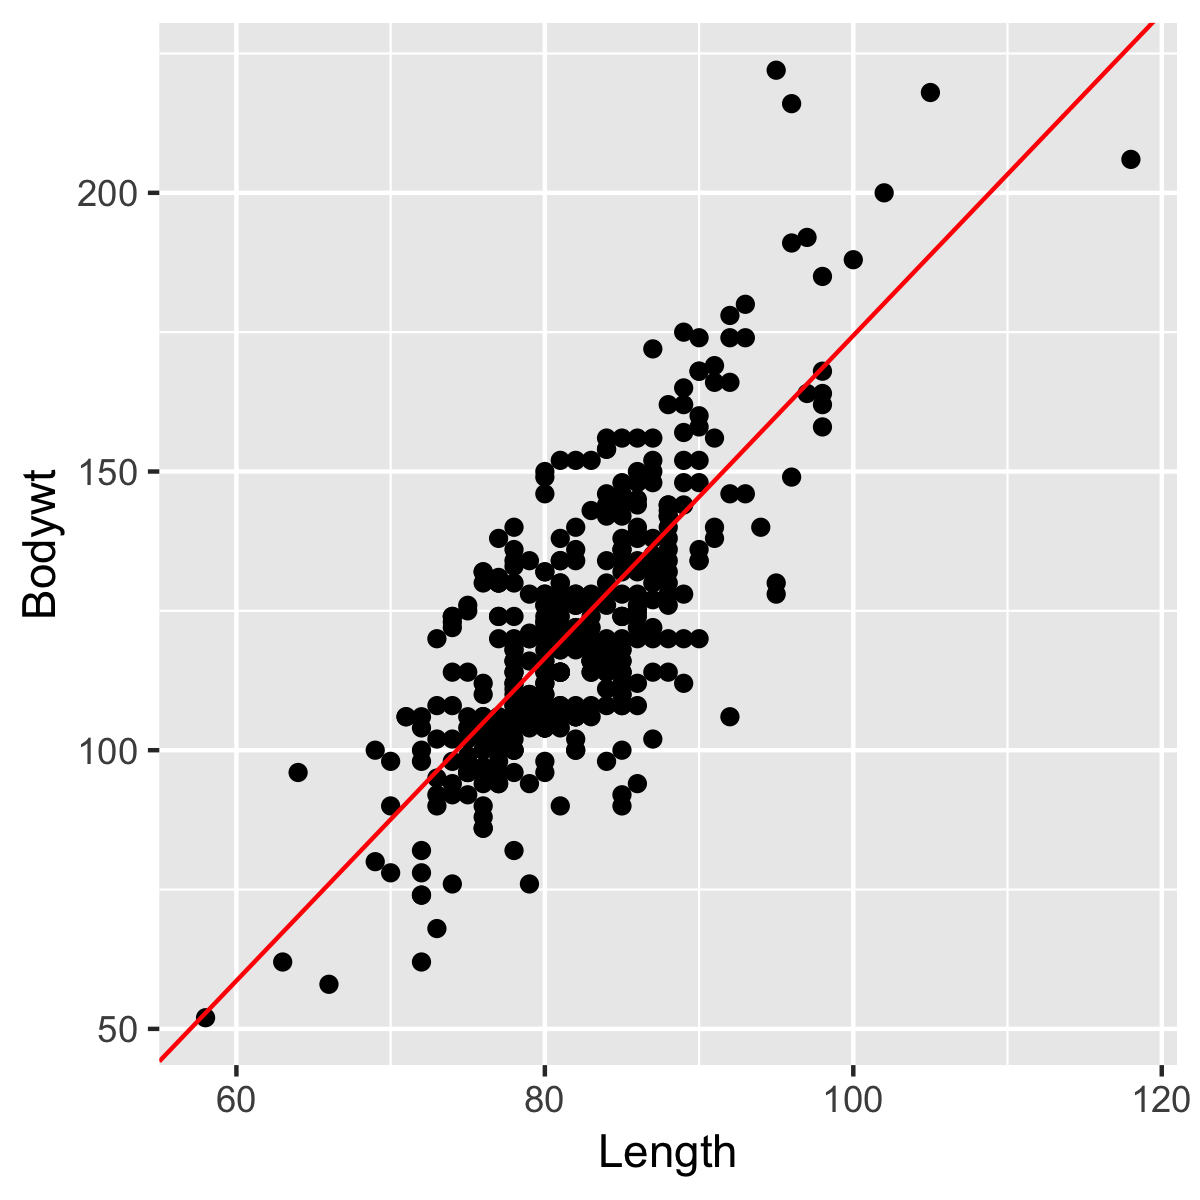
\includegraphics{lecture2_in_class_files/figure-latex/unnamed-chunk-7-1.pdf}

\begin{Shaded}
\begin{Highlighting}[]
\KeywordTok{ggplot}\NormalTok{(}\DataTypeTok{data =}\NormalTok{ df, }\KeywordTok{aes}\NormalTok{(}\DataTypeTok{x =}\NormalTok{ color)) }\OperatorTok{+}\StringTok{ }\KeywordTok{geom_bar}\NormalTok{() }
\end{Highlighting}
\end{Shaded}

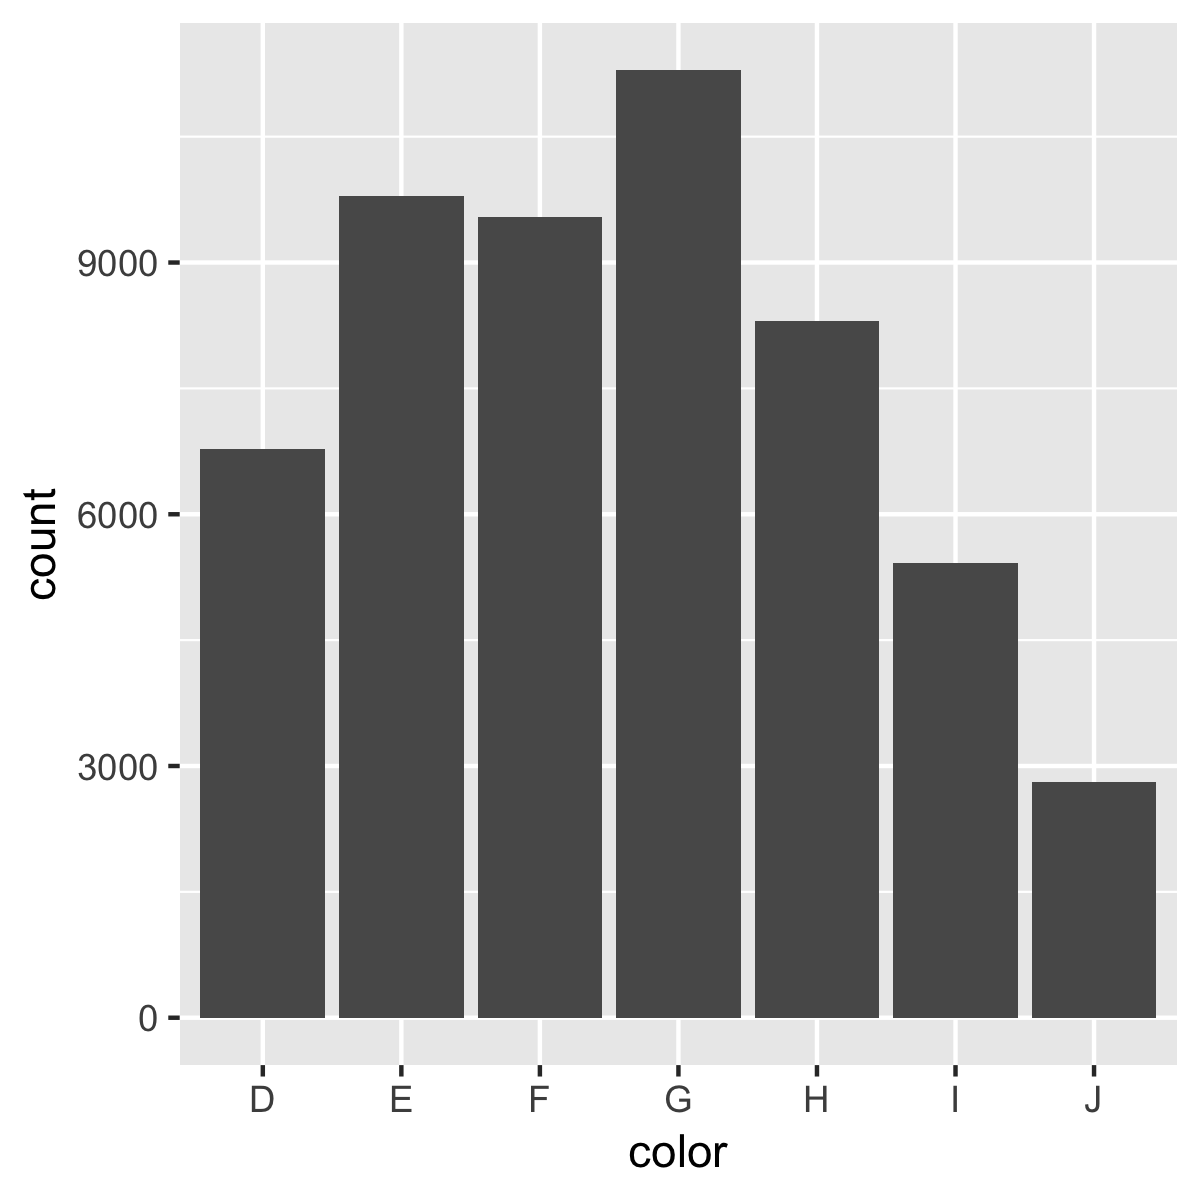
\includegraphics{lecture2_in_class_files/figure-latex/unnamed-chunk-8-1.pdf}

\begin{Shaded}
\begin{Highlighting}[]
\KeywordTok{ggplot}\NormalTok{(df, }\KeywordTok{aes}\NormalTok{(cut)) }\OperatorTok{+}\StringTok{ }\CommentTok{## can omit 'data = ' and 'x = '}
\StringTok{  }\KeywordTok{geom_bar}\NormalTok{() }\OperatorTok{+}
\StringTok{  }\KeywordTok{facet_wrap}\NormalTok{(}\OperatorTok{~}\NormalTok{color)}
\end{Highlighting}
\end{Shaded}

\includegraphics{lecture2_in_class_files/figure-latex/unnamed-chunk-8-2.pdf}

\begin{Shaded}
\begin{Highlighting}[]
\KeywordTok{ggplot}\NormalTok{(df, }\KeywordTok{aes}\NormalTok{(cut, }\DataTypeTok{fill =}\NormalTok{ clarity)) }\OperatorTok{+}\StringTok{ }\CommentTok{## can omit 'data = ' and 'x = '}
\StringTok{  }\KeywordTok{geom_bar}\NormalTok{() }\OperatorTok{+}
\StringTok{  }\KeywordTok{facet_wrap}\NormalTok{(}\OperatorTok{~}\NormalTok{color) }\OperatorTok{+}
\StringTok{  }\KeywordTok{theme}\NormalTok{(}\DataTypeTok{axis.text.x =} \KeywordTok{element_text}\NormalTok{(}\DataTypeTok{angle =} \DecValTok{-90}\NormalTok{, }\DataTypeTok{hjust =} \DecValTok{0}\NormalTok{))}
\end{Highlighting}
\end{Shaded}

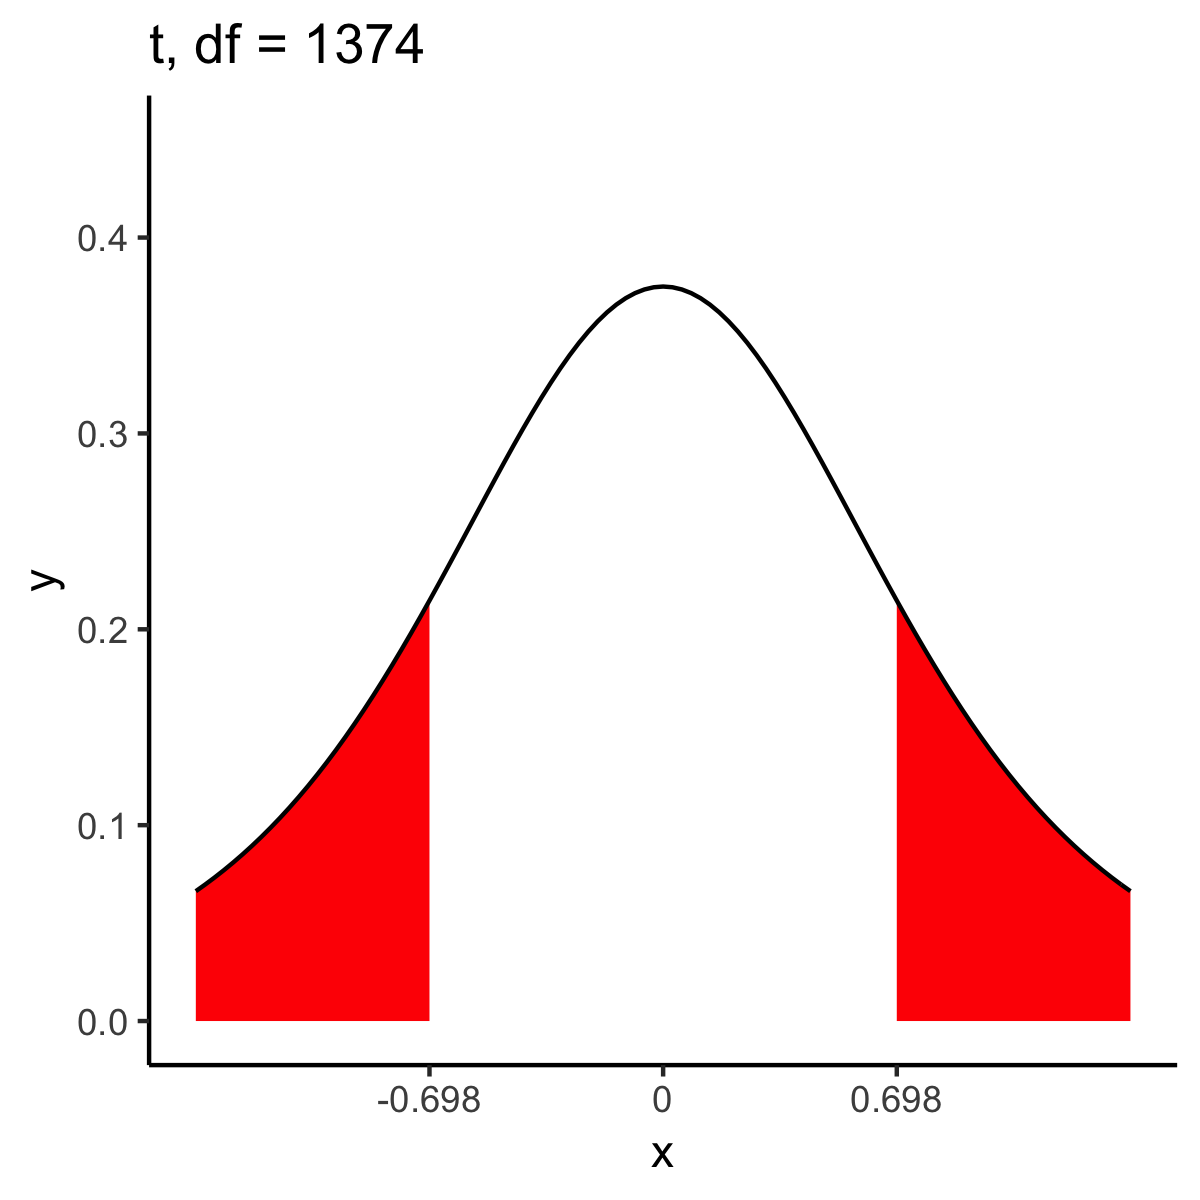
\includegraphics{lecture2_in_class_files/figure-latex/unnamed-chunk-9-1.pdf}

\begin{Shaded}
\begin{Highlighting}[]
\KeywordTok{ggplot}\NormalTok{(df, }\KeywordTok{aes}\NormalTok{(carat)) }\OperatorTok{+}
\StringTok{  }\KeywordTok{geom_histogram}\NormalTok{(}\DataTypeTok{bins =} \DecValTok{30}\NormalTok{)}
\end{Highlighting}
\end{Shaded}

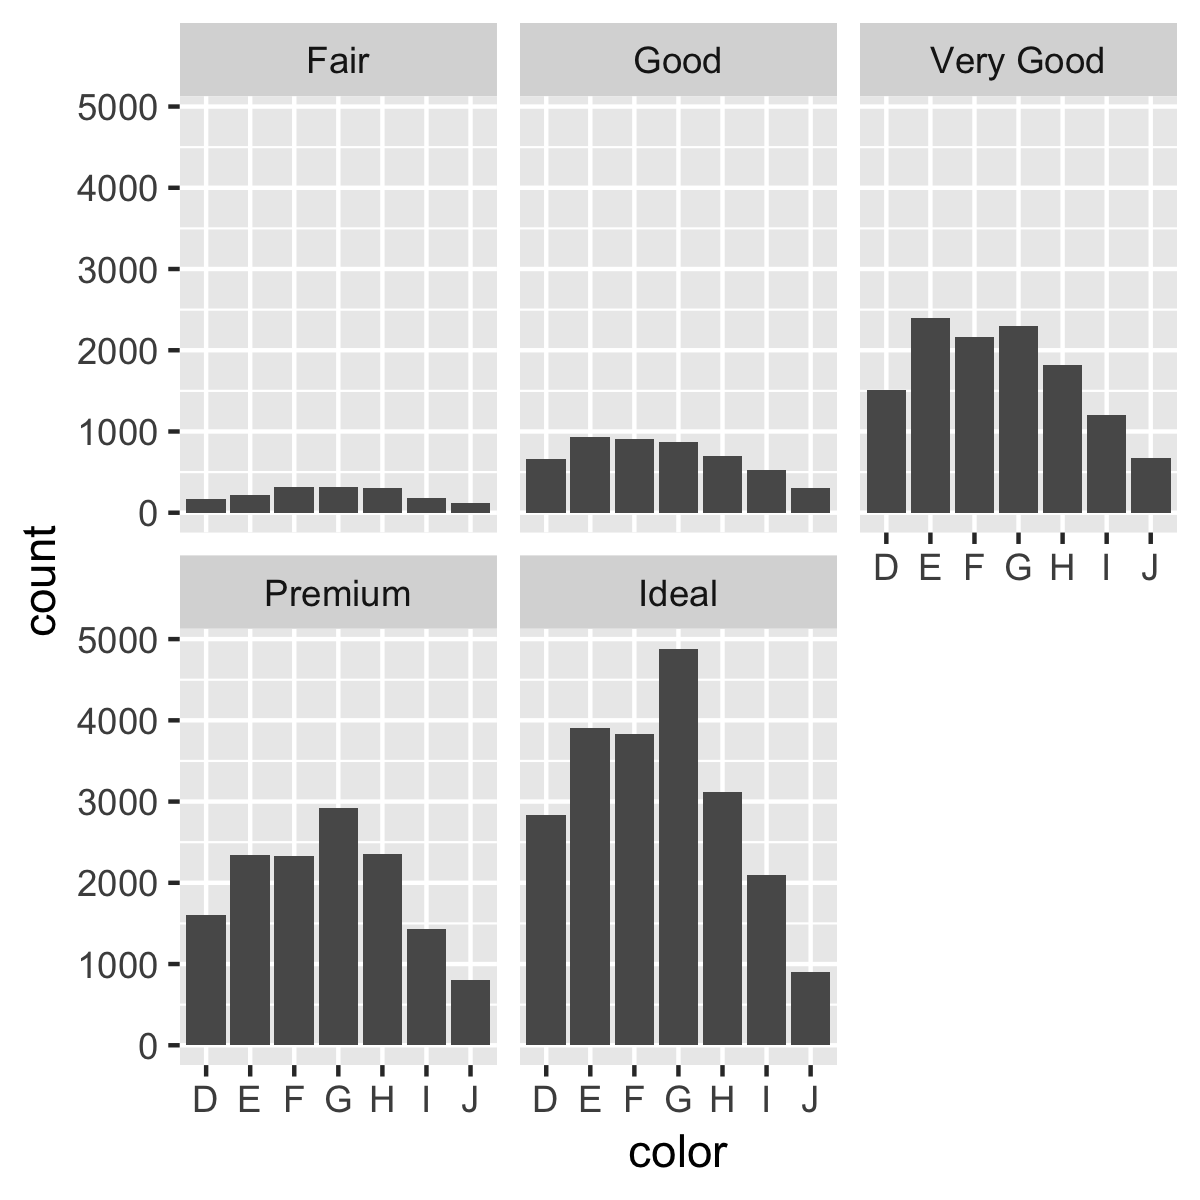
\includegraphics{lecture2_in_class_files/figure-latex/unnamed-chunk-10-1.pdf}

\begin{Shaded}
\begin{Highlighting}[]
\NormalTok{?quantile}

\KeywordTok{sqrt}\NormalTok{(}\FloatTok{5.546511}\NormalTok{)}
\end{Highlighting}
\end{Shaded}

\begin{verbatim}
## [1] 2.355103
\end{verbatim}

\end{document}
